\section{Ergebnisse}
\label{sec:ergebnisse}

\subsection*{Ausbeute}

Mit den eingewogenen \SI{25}{\gram} Nelkenblüten und der Probenmasse von \SI{3,87}{\gram} berechnet sich in Gleichung \ref{gl:ausbeute} der Naturstoffgehalt für diese Versuchsdurchführung.
\begin{flalign}
	\label{gl:ausbeute}
	\eta 	&= \frac{m_{\text{Probe}}}{m_{\text{Naturstoff}}}\\
				&= \frac{\SI{3,87}{\gram}}{\SI{25,03}{\gram}}\\
				&=	\underline{\SI{15,46}{\percent}}
\end{flalign}

\subsection*{Gaschromatografie mit Massenspektren} 
In den Abbildungen \ref{fig:chroma_ms} und \ref{fig:chroma_fid} sind die aufgenommenen Chromatogramme des Nelkenöls dargestellt. In beiden Abbildungen sind drei Peaks bei ähnlichen Retentionszeiten zu erkennen. Diese stehen für die drei Hauptverbindungen des Nelkenöls. Es lassen sich Retentionszeiten der Peaks bei \SI{26,43}{\minute}, \SI{28,15}{\minute} und \SI{30,24}{\minute} ablesen. Es lassen sich Abweichungen der Chromatogramme ab der 2. Nachkommastelle feststellen.

\begin{figure}[h!]
	\begin{minipage}{0.45\textwidth}
		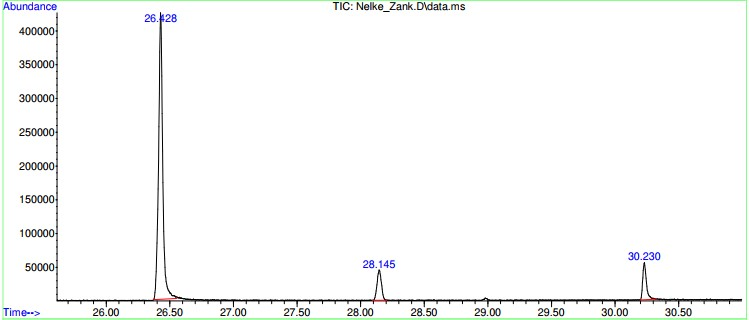
\includegraphics[width=0.95\textwidth]{img/chroma_ms}
		\caption{Chromatogramm mit Massenspektrometrie-Kopplung des Nelkenöls}\label{fig:chroma_ms}
	\end{minipage}\hfill
	\begin{minipage}{0.45\textwidth}
		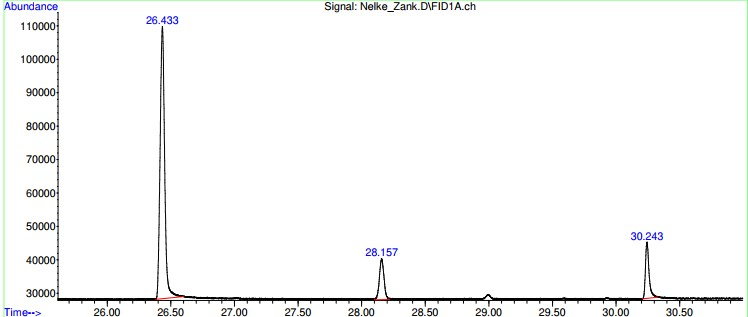
\includegraphics[width=0.95\textwidth]{img/chroma_fid}
		\caption{Chromatogramm mit Flammenionisationsdetektor- Kopplung des Nelkenöls}\label{fig:chroma_fid}
	\end{minipage}\hfill
\end{figure}
\FloatBarrier

In den Abbildungen \ref{fig:ms_164} bis \ref{fig:ms_206} sind die Massenspektren für die Retentionszeiten aus den Chromatogrammen dargestellt.

\begin{figure}[h!]
	\centering
	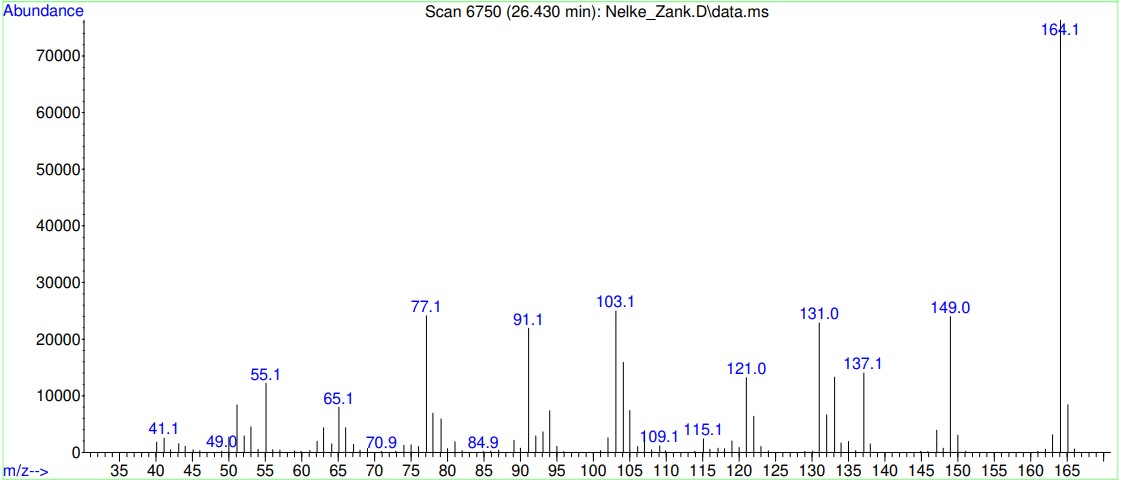
\includegraphics[width=0.85\textwidth]{img/ms_164}
	\caption{Massenspektrogramm für Verbindung mit Retentionszeit \SI{26,43}{\minute}}
	\label{fig:ms_164}
\end{figure}
\FloatBarrier
\begin{figure}[h!]
	\centering
	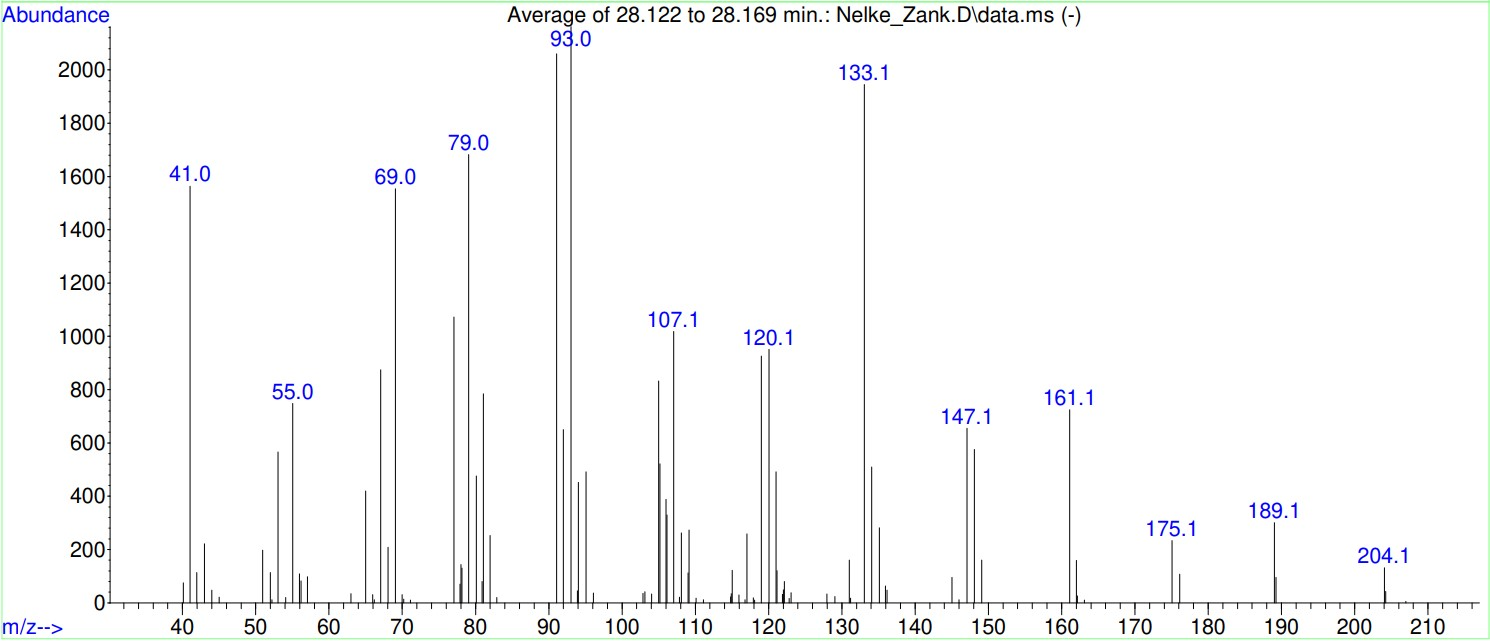
\includegraphics[width=0.85\textwidth]{img/ms_204}
	\caption{Massenspektrogramm für Verbindung mit Retentionszeit \SI{28,15}{\minute}}
	\label{fig:ms_204}
\end{figure}
\FloatBarrier
\begin{figure}[h!]
	\centering
	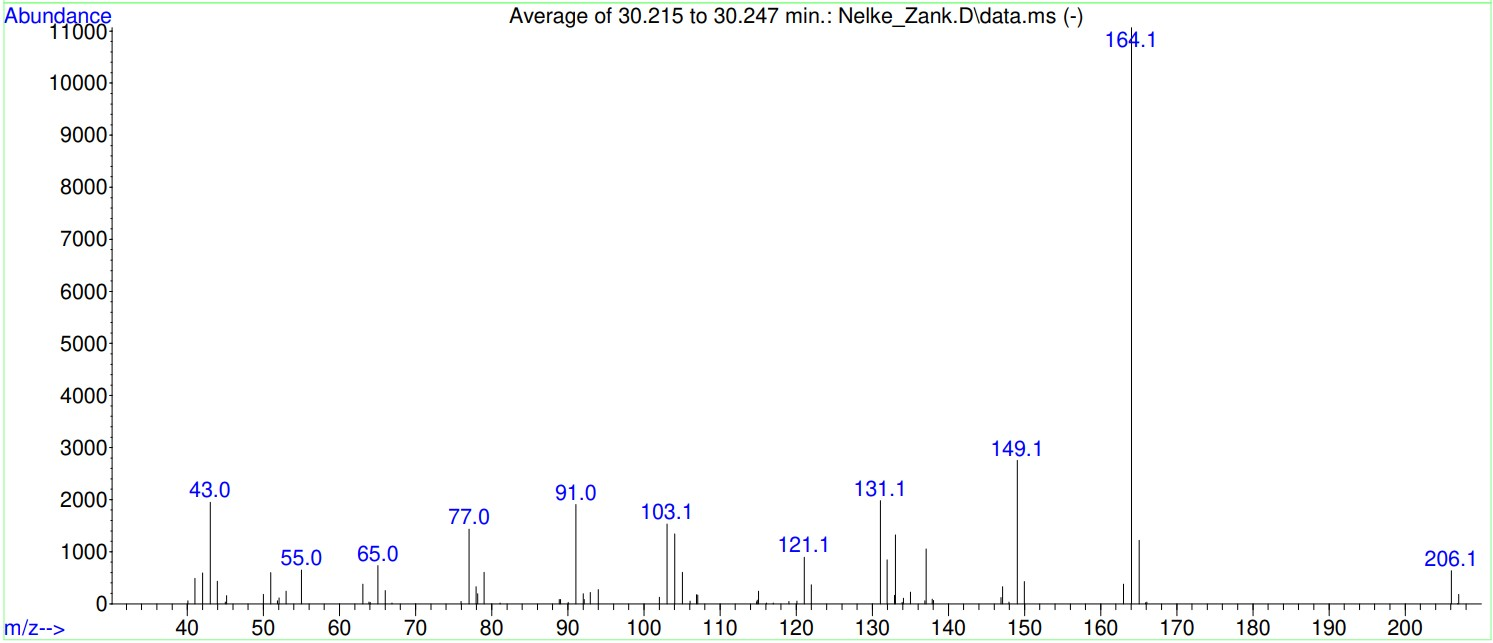
\includegraphics[width=0.85\textwidth]{img/ms_206}
	\caption{Massenspektrogramm für Verbindung mit Retentionszeit \SI{30,24}{\minute}}
	\label{fig:ms_206}
\end{figure}
\FloatBarrier

In Abbildung \ref{fig:ms_164} ist die maximal gemessene molare Masse \SI{164}{\gram \per \mole} für eine Retentionszeit von \SI{26,43}{\minute}. Dementsprechend besitzt die Verbindung im ersten, höchsten Peak eine molare Masse von \SI{164}{\gram \per \mole}.\\
\newpage
In Abbildung \ref{fig:ms_204} ist die maximal gemessene molare Masse \SI{204}{\gram \per \mole} für eine Retentionszeit von \SI{28,15}{\minute}. Dementsprechend besitzt die Verbindung im zweiten Peak eine molare Masse von \SI{204}{\gram \per \mole}.\\
In Abbildung \ref{fig:ms_206} ist die maximal gemessene molare Masse \SI{206}{\gram \per \mole} für eine Retentionszeit von \SI{30,24}{\minute}. Dementsprechend besitzt die Verbindung im dritten Peak eine molare Masse von \SI{206}{\gram \per \mole}.

\subsection*{Zusammensetzung}
Das Auswertungsprogramm für die Chromatogramme gab, wie in Abbildung \ref{fig:zusammen} zu sehen, über eine Berechnung der Flächen unter den Peaks der jeweiligen Verbindungen an, zu welchen Anteilen diese Prozentual im Öl vertreten sind.

\begin{figure}[h!]
	\centering
	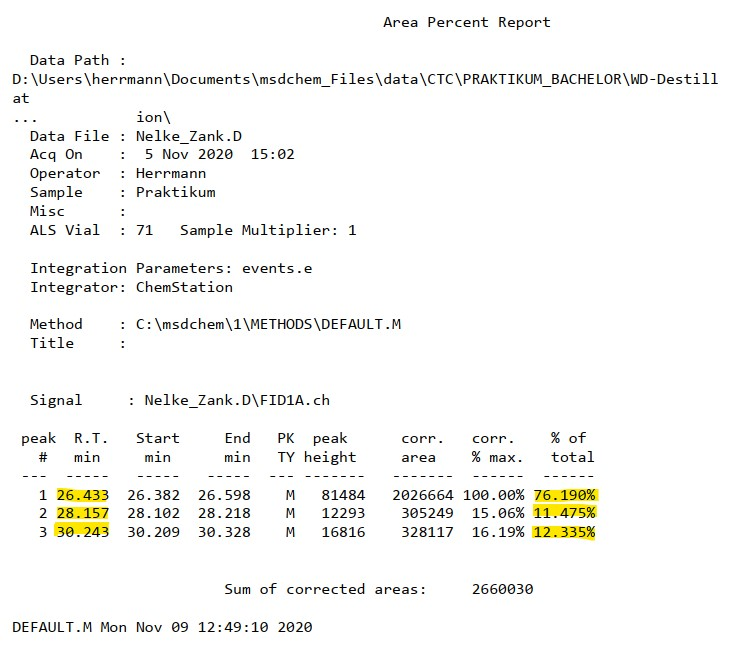
\includegraphics[width=0.85\textwidth]{img/zusammen}
	\caption{computergestützte Auswertung der Chromatogramme}
	\label{fig:zusammen}
\end{figure}
\FloatBarrier

In Tabelle \ref{tab:zusammen} sind zusammengetragenen Ergebnisse noch einmal zusammengefasst:

\begin{table}[h!]
	\renewcommand*{\arraystretch}{1.2}
	\centering
	\rowcolors{2}{white}{gray!25}
	\caption{Zusammengefasste Ergebnisse der Gaschromatografie und der \mbox{Massenspektroskopie}}
	\label{tab:zusammen}
	\resizebox{10.5cm}{!}{
		\begin{tabulary}{1.0\textwidth}{C|C|C|C}
			\hline
			\textbf{Verbindung} & \textbf{Retentionszeit} $\left[\si{\minute}\right]$& \textbf{Molare Masse} $\left[\si{\gram \per \mole}\right]$&\textbf{Anteil} $\left[\si{\percent}\right]$\\
			\hline
			Verbindung 1 & 26,43 & 164 & 76,2\\
			Verbindung 2 & 28,15 & 204 & 11,5\\
			Verbindung 3 & 30,24 & 206 & 12,3\\
			\hline      
	\end{tabulary}}
\end{table}%
\FloatBarrier




